\chapter{Moto Rigido Tridimensionale}\label{3d}
\section{Il Moto nelle Tre Dimensioni dello Spazio}
\begin{wrapfigure}{r}{0.45\textwidth}
\centering{
      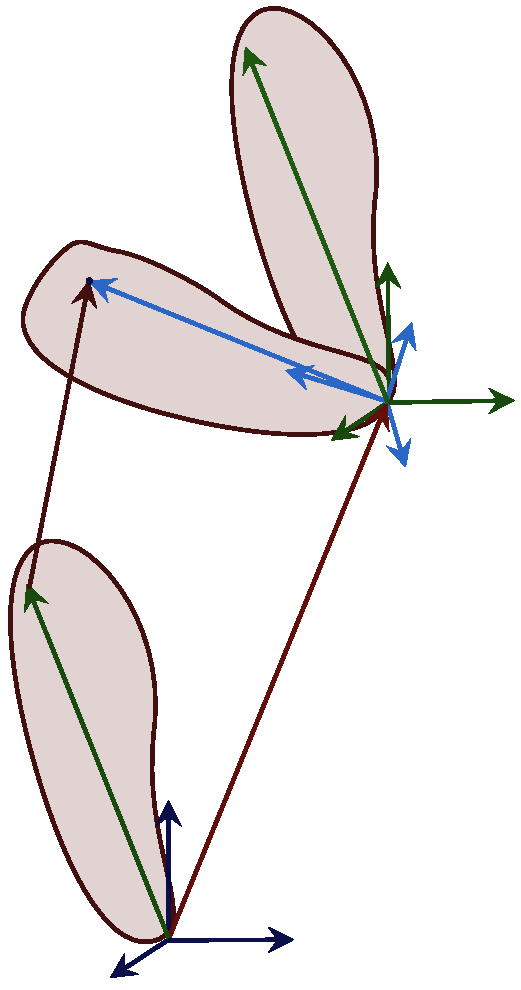
\includegraphics[width=0.40\textwidth]{part3/3d/FIG/f11_app11.pdf}}
\begin{picture}(0,0)(118,23)
\scriptsize{
\put(37.5,285){$P$}
\put(-11,221){$P$}
\put(-18,133){$P$}
\put(14,29){$\bm {G} \equiv \bm \Gamma$}
\put(74,161.5){${\bm \Lambda}$}
\put(94,190){${\bm J}$}
\put(45,100){${{\bm s}}$}
\put(-14,165){${\bm s}_{\scriptscriptstyle{P}}$}
\put(-3,89){${\bm z}_{\scriptscriptstyle{P}}$}
\put(53,249){${\bm z}_{\scriptscriptstyle{P(J)}}$}
\put(20,197){${\bm z}_{\scriptscriptstyle{P(\Lambda)}}$}
\put(1,22){${{\bm e}_1}$}
\put(50,32){${{\bm e}_2}$}
\put(18,74){${{\bm e}_3}$}
\put(84,167){${{\bm e}_1}_{R}$}
\put(85,206){${{\bm e}_2}_{R}$}
\put(45,187){${{\bm e}_3}_{R}$}
}
\end{picture}
	\caption{\em Moto tridimensionale di una clavetta.}
     \label{fig:f11_app11}
\end{wrapfigure}
Il moto di un corpo  nello
spazio tridimensionale rappresenta il
caso generale della {\em cinematica
del corpo rigido}\index{cinematica del corpo rigido}.
Lo si studia con lo scopo,
come avviene nel caso piano, di mettere in relazione tra loro
le varie grandezze cinematiche che vi partecipano,
riferendole, in generale, a un osservatore fisso.
Costui sar\`a nel seguito surrogato
da una {\em terna orientata}\index{terna!orientata} 
$\bm{G}$.
Ci occuperemo, in prima battuta (e in coda), di uno spostamento finito,
del quale sar\`a protagonista
il nostro corpo rigido, che nelle figure \`e rappresentato da una clavetta.
Tale spostamento
far\`a passare la clavetta da una posizione iniziale, nella quale
la terna $\bm \Gamma$, ad essa rigidamente collegata, coincide con
la terna $\bm G$, a una seconda posizione,
nella quale la terna $\bm \Gamma$
si trover\`a in un altro punto dello spazio e avr\`a 
un diverso orientamento: in questa nuova posizione, ci riferiremo ad essa
col nome ${\bm \Lambda}$.

\noindent Consideriamo le terne 
$\bm G$
e $\bm \Gamma$
costituite ciascuna 
da tre versori ortogonali, 
come in figura \ref{fig:f11_app11},
che si possono  
assumere quali {\em vettori di base} per
gli spazi fisso e mobile.
Come abbiamo gi\`a accennato, la terna $\bm{ \Gamma}$, vincolata alla clavetta,
accompagner\`a quest'ultima nei suoi spostamenti e un osservatore
ad essa solidale vedr\`a il punto $P$, appartenente alla clavetta stessa, 
stare fermo.
Evidenziamo che, una volta nota la posizione dell'origine di $\bm \Gamma$,
si potr\`a conoscere la posizione di tutti i punti della clavetta, cio\`e
dello spazio mobile,
conoscendo la posizione di un suo punto generico,
che abbiamo gi\`a indicato con $P$. 
Consideriamo ora lo spostamento generico della clavetta
come idealmente composto da due distinte fasi.
Durante la prima di queste due fasi portiamo semplicemente 
la terna $\bm \Gamma$ a sovrapporsi alla terna $\bm J$.
La seconda fase dello spostamento
vede invece il vettore 
${{\bm z}}_{\scriptscriptstyle{P(J)}}$ andare a coincidere con 
${{\bm z}}_{\scriptscriptstyle{P(\Lambda)}}$, e $\bm J$
stessa sovrapporsi a $\bm \Lambda$, lasciando fisso il centro di $\bm J$.
Pertanto, queste due operazioni
forniscono una ``ricetta''
per conoscere la posizione ``assoluta'' di $P$.
Ma esse presentano difficolt\`a di grado diverso.
Infatti, per portare la terna $\bm\Gamma$ nella terna $\bm J$
baster\`a aggiungere a tutti i punti
dello spazio mobile,
riferiti a $\bm G$, il vettore
${\bm{s}}$.  Invece, per orientare gli assi
di $\bm J$ in modo che essi si sovrappongano a quelli
di $\bm \Lambda$ si intuisce che 
occorrer\`a
operare mediante ``opportune rotazioni'' della stessa terna $\bm J$:
ma quali sono queste rotazioni?
Lasciamo questa domanda in sospeso e rispolveriamo qualche strumento
di cui ci siamo dotati
seguendo il corso di Algebra Lineare.  

\noindent Consideriamo la trasformazione
del vettore 
${{\bm z}}_{\scriptscriptstyle{P(J)}}$ che lo porta a coincidere col vettore
${{\bm z}}_{\scriptscriptstyle{P(\Lambda)}}$.
A tale scopo, chiamiamo con $\bm R$ un operatore di trasformazione dei 
vettori nello spazio tale per cui 
\begin{equation}
{{\bm z}}_{\scriptscriptstyle{P(\Lambda)}}=
{\bm R}{\bm z}_{\scriptscriptstyle{P(J)}}\,.
\label{e11_app11}
\end{equation}
\noindent Affinch\'e $\bm{R}$ rappresenti una rotazione rigida, la sua applicazione a
due vettori qualsiasi dovr\`a 
lasciare inalterato l'angolo tra le direzioni dei due vettori stessi;
inoltre essa non dovr\`a n\'e dilatare
n\'e restringere i loro moduli. Tutto questo, sinteticamente, si esprime dicendo
che la trasformazione $\bm R$
 deve mantenere invariante il {\em prodotto scalare}
tra due vettori qualsiasi, prima e dopo la sua applicazione\footnote
{
Ci siamo riferiti all'operatore $\bm R$ come, appunto, a un'operazione
sui vettori dello spazio tridimensionale. A questo operatore, come anche
ai vettori sui quali esso opera, compete ovviamente
una rappresentazione matriciale
legata ai vettori di base: matrici $1\times3$ saranno le rappresentazioni dei vettori,
mentre la rappresentazione dell'operatore $\bm R$ consister\`a in una matrice
$3\times3$. Speriamo di non ingenerare dubbi nei lettori in conseguenza della
scelta di mantenere inalterati i nomi dei vettori, degli operatori e
delle loro rappresentazioni.
}.
Quindi, posto che, tramite $\bm{R}$,
 $\bm{v} \rightarrow {\bm{v}}_R$ e  $\bm{u} \rightarrow {\bm{u}}_R$,
possiamo scrivere l'uguaglianza (tra le rappresentazioni di questi oggetti)
\begin{equation}
{{\bm{u}}_R}^T{\bm{v}}_R={\bm{u}}^T{\bm{R}}^T{\bm{R}}{\bm{v}}\,.
\label{e12_app11}
\end{equation}
\noindent Ma per quanto appena affermato circa l'invarianza del prodotto scalare tra
due vettori dovr\`a essere
\begin{equation}
\bm{R}^T\bm{R}={\bm{I}}\,.
\label{e13_app11}
\end{equation}
\noindent Quando la trasposta (coniugata, nel caso di matrici complesse) di una matrice si comporta come la sua inversa
sappiamo, sempre dall'Algebra Lineare, che tale
matrice 
\`e {\em unitaria} e che il suo determinante vale uno. Vale poi anche
\begin{equation}
\bm{R}\bm{R}^T={\bm{I}}\,.
\label{e14_app11}
\end{equation}
\noindent Pertanto, se $\bm{R}$ rispetta la \ref{e13_app11}, essa ruota lo spazio a cui si applica
e lascia invariati gli angoli e le dimensioni degli oggetti.
Restringendo le nostre considerazioni a uno spazio con solo due 
dimensioni, giusto per proporre qualcosa di facilmente verificabile
 a quei lettori
poco desiderosi di accordare tutta questa confidenza all'Algebra Lineare,
tale matrice assume la forma
\begin{equation}
{\bm R}=\left( \begin{array}{cc}
\cos \theta & -\sin \theta\\ 
\sin \theta & \cos \theta
\end{array}
\right)
\,,
\label{e15_app11}
\end{equation}
 \noindent dove
$\theta$ rappresenta l'unico possibile angolo di rotazione nel piano.
\noindent La situazione \`e concettualmente analoga, bench\'e 
sia pi\`u complessa, nello spazio
tridimensionale. 
In questo caso infatti la matrice\footnote{
Sarebbe ${\bm R}^{-1}$ ad essere cos\`i composta, ma
${\bm R}^T={\bm R}^{-1}$.
}
${\bm{R}}^T$,
formata dalle colonne della
rappresentazione dei vettori $\left({{\bm e}_1}_{R},{{\bm e}_2}_{R},
{{\bm e}_3}_{R}\right)$ sulla base $\left(\bm{e}_1, \bm{e}_2, \bm{e}_3\right)$,
\`e tale per cui
\begin{equation}
({{\bm e}_1}_{R},{{\bm e}_2}_{R}, {{\bm e}_3}_{R})
= {\bm R}\cdot
(\bm{e}_1, \bm{e}_2, \bm{e}_3)
\,,
\label{eq:rot}
\end{equation}
\noindent e, dato un ben preciso orientamento di ${\bm \Lambda}$,
essa pu\`o essere ottenuta seguendo diversi percorsi.
Fatta salva quindi l'unicit\`a della matrice $\bm R$, esistono diverse
composizioni di rotazioni successive della terna $\bm J$ che la portano
a coincidere con $\bm \Lambda$. Tali procedimenti di rotazione
tengono naturalmente conto degli angoli via via coinvolti e prendono
il nome dal loro primo proponente ovvero dal particolare ambito nel quale il
loro uso \`e prevalente.
Abbiamo cos\`i gli {\em angoli di Eulero}\index{angoli!di Eulero}: {\em
precessione}\index{precessione}, {\em nutazione}\index{nutazione} e 
{\em rotazione}\index{rotazione}, normalmente indicati coi simboli
$\theta$, $\phi$  e $\psi$,
\cite{whittaker}, pagg. 8--12, gli {\em angoli di Cardano}\index{angoli!di Cardano}, meno noti e non molto dissimili da quelli di {\em Eulero} e talvolta
chiamati col nome di {\em angoli nautici}\index{angoli!nautici} e
spesso indicati coi nomi
di {\em imbardata}\index{imbardata}, {\em rollio}\index{rollio} e 
{\em beccheggio}\index{beccheggio}, e altri ancora.

\section{Rotazioni Infinitesimali}

\noindent Se restringiamo il campo delle rotazioni a quelle
infinitesimali, che ormai sappiamo essere
strettissime parenti delle velocit\`a angolari, una volta rapportate 
al tempo infinitesimale durante il quale esse si manifestano,
le cose marciano con maggior semplicit\`a.
Consideriamo la \ref{e11_app11} e differenziamola:
\begin{equation}
{\rm d}{\bm{z}}_{\scriptscriptstyle{P(\Lambda)}}=
\left({\rm d}\bm{R}\right){\bm{z}}_{\scriptscriptstyle{P(J)}}+
\bm{R}\left({\rm d}{\bm{z}}_{\scriptscriptstyle{P(J)}}\right)\,.
\label{e16_app11}
\end{equation}
\noindent Si nota che, in virt\`u della condizione di corpo rigido, 
${\rm d}{\bm{z}}_{\scriptscriptstyle{P(J)}}=0$, perch\'e la posizione del
punto $\bm P$ nel sistema di riferimento mobile con la clavetta \`e costante.
Dobbiamo quindi osservare attentamente il termine 
$\left({\rm d}\bm{R}\right){\bm{z}}_{\scriptscriptstyle{P(J)}}$,
nel quale compare il differenziale della matrice di rotazione $\bm R$. 
Premettiamo che le prossime mosse potrebbero apparire un po' artificiose,
bench\'e il loro
senso sia contenuto nel seguente {\em modus operandi}: costruire una
``matrice derivata'' che operi sul vettore che identifica il punto $P$
{\em gi\`a ruotato}, 
${\bm{z}}_{\scriptscriptstyle{P(\Lambda)}}$,
anzich\'e su
${\bm{z}}_{\scriptscriptstyle{P(J)}}$.
\begin{wrapfigure}{r}{0.45\textwidth}
\centering{
      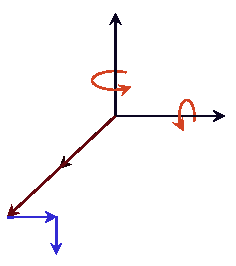
\includegraphics[width=0.38\textwidth]{part3/3d/FIG/f12_app11.pdf}
}
\begin{picture}(40,25)(18,10)
\scriptsize{
\put(8,87){${\bm{e'}_1}$}
\put(93,114){${\bm{e'}_2}$}
\put(38,185){${\bm{e'}_3}$}
\put(14,134){${\rm d}\phi_{{\scriptscriptstyle{1,2}}}$}
\put(74,137){${\rm d}\phi_{{\scriptscriptstyle{3,1}}}$}
\put(-9.5,69.5){${\rm d}\phi_{{\scriptscriptstyle{1,2}}}x$}
\put(4,50){${\rm d}\phi_{{\scriptscriptstyle{3,1}}}x$}
\put(-33,69){$\bm x$}
}
\end{picture}
\vskip -10mm
	\caption{\em Rotazioni infinitesimali.}
     \label{fig:f12_app11}
\end{wrapfigure}
Per la propriet\`a di $\bm R$ espressa da \ref{e13_app11}, riscriviamo
la \ref{e16_app11} interponendo tra i due fattori la matrice identit\`a
$\bm{R}^T\bm{R}$ ottenendo cos\`i la seguente relazione:
\begin{equation}
{\rm d}{\bm{z}}_{\scriptscriptstyle{P(\Lambda)}}=
\left({\rm d}\bm{R}\right)\bm{R}^T\bm{R}{\bm{z}}_{\scriptscriptstyle{P(J)}}
\,,
\label{e17_app11}
\end{equation}
\noindent cio\`e
\begin{equation}
{\rm d}{\bm{z}}_{\scriptscriptstyle{P(\Lambda)}}=
\left({\rm d}\bm{R}\right)\bm{R}^T{\bm{z}}_{\scriptscriptstyle{P(\Lambda)}}
\,.
\label{e18_app11}
\end{equation}
\noindent Ma derivando la \ref{e14_app11}, notiamo che
\begin{equation}
\left({\rm d}\bm{R}\right)\bm{R}^T+
\bm{R}\left({\rm d}\bm{R}\right)^T=0\,,
\label{e19_app11}
\end{equation}
\noindent o anche

\vskip 1mm
\begin{equation}
\left({\rm d}\bm{R}\right)\bm{R}^T=
-\bm{R}\left({\rm d}\bm{R}\right)^T\,,
\label{e110_app11}
\end{equation}
\noindent La matrice $\left({\rm d}\bm{R}\right)\bm{R}^T$ \`e quindi una matrice
antisimmetrica e infinitesimale (prodotto di una matrice infinitesimale
per una finita) che chiameremo 
${\rm d}\bm{\Phi}=\left({\rm d}\bm{R}\right)\bm{R}^T$. \`E facile convincersi che tale matrice
contiene i tre angoli infinitesimali
di rotazione nei tre piani individuati da ciascuna coppia di vettori di base di
$\bm \Lambda$: 
%$\left(\bm{e'}_1, \bm{e'}_2, \bm{e'}_3\right)$:
\begin{equation}
{\rm d}{\bm\Phi}=\left( \begin{array}{ccc}
0 & -{\rm d}\phi_{{\scriptscriptstyle{1,2}}} & {\rm d}\phi_{{\scriptscriptstyle{3,1}}}\\
{\rm d}\phi_{{\scriptscriptstyle{1,2}}} & 0 & -{\rm d}\phi_{{\scriptscriptstyle{2,3}}}\\
-{\rm d}\phi_{{\scriptscriptstyle{3,2}}} & {\rm d}\phi_{{\scriptscriptstyle{2,3}}} & 0\\
\end{array}
\right)
\,.
\label{e111_app11}
\end{equation}
\noindent Ai suoi elementi abbiamo dato nomi evocativi e segni disparati: conviene
ora fare una prova per renderci conto se tali nomi e tali segni siano o meno
opportuni.
Applichiamo la matrice ${\rm d}\bm \Phi$ al vettore $\bm x$ di modulo costante rappresentato
in figura \ref{fig:f12_app11}, la cui giacitura coincide con quella del
versore $\bm{e'}_1$ con lo scopo di trovare ${\rm d}\left(\bm{x}\right)$.
Avremo
\begin{equation}
{\rm d}
 \left( \begin{array}{c}
x \\ 
0 \\ 
0 \\
\end{array}
\right)=
\left( \begin{array}{ccc}
0 & -{\rm d}\phi_{{\scriptscriptstyle{1,2}}} & {\rm d}\phi_{{\scriptscriptstyle{3,1}}}\\
{\rm d}\phi_{{\scriptscriptstyle{1,2}}} & 0 & -{\rm d}\phi_{{\scriptscriptstyle{2,3}}}\\
-{\rm d}\phi_{{\scriptscriptstyle{3,1}}} & {\rm d}\phi_{{\scriptscriptstyle{2,3}}} & 0\\
\end{array}
\right)
 \left( \begin{array}{c}
x \\ 
0 \\ 
0 \\
\end{array}
\right)=
 \left( \begin{array}{c}
0 \\
{\rm d}\phi_{{\scriptscriptstyle{1,2}}}x \\
-{\rm d}\phi_{{\scriptscriptstyle{3,1}}}x \\
\end{array}
\right)
\,,
\label{e112_app11}
\end{equation}
\vskip 2mm
\noindent che, confrontato con la figura \ref{fig:f12_app11}, ci conforta alquanto.
Il procedimento si pu\`o ripetere (con successo) per i vettori che giacciano
sulle altre due direzioni, cos\`i avremo provato ``alla buona'' che
gli elementi della matrice
${\rm d}\bm \Phi$ sono le rotazioni infinitesime.
Dividendo poi tale matrice per ${\rm d}t$ si ottiene la matrice (finita) delle
velocit\`a angolari
\begin{equation}
{\bm\Omega}=\left( \begin{array}{ccc}
0 & -\omega{{\scriptscriptstyle{1,2}}} & \omega{{\scriptscriptstyle{3,1}}}\\
\omega{{\scriptscriptstyle{1,2}}} & 0 & -\omega{{\scriptscriptstyle{2,3}}}\\
-\omega{{\scriptscriptstyle{3,1}}} & \omega{{\scriptscriptstyle{2,3}}} & 0\\
\end{array}
\right)
\,.
\label{e113_app11}
\end{equation}
\noindent Siamo ora in grado di rispondere al nostro quesito iniziale, cio\`e di conoscere
posizione e velocit\`a del punto $P$
sapendo come si muove la terna $\bm \Lambda$. Per gli spostamenti avremo
\begin{equation}
{\bm s}_{\scriptscriptstyle{P}}=
{{\bm s}}+
{\bm R}{\bm z}_{\scriptscriptstyle{P}}-
{\bm z}_{\scriptscriptstyle{P}}\,,
\label{e114_app11}
\end{equation}
\noindent e per quanto riguarda le velocit\`a
\begin{equation}
{\bm v}_{\scriptscriptstyle{P}}=
{\bm v}_{\scriptscriptstyle\Lambda}+
{\bm \Omega}{\bm z}_{\scriptscriptstyle{P}}\,.
\label{e115_app11}
\end{equation}

\section{Asse del Mozzi e Altre Considerazioni}
\noindent Ci chiediamo a questo punto se, come nel caso piano, vi siano dei punti
o dei luoghi privilegiati che,
a fronte del movimento tridimensionale della clavetta,
non subiscono spostamenti, oppure siano sottoposti
soltanto a movimenti particolarmente semplici.
Come ora sappiamo, l'equazione \ref{e114_app11} fornisce lo spostamento di un
generico punto dello {\em spazio mobile}.
Imponendo che lo spostamento di un punto incognito,
che chiameremo
$Q$, sia nullo
\begin{equation}
0=
{{\bm s}}+
{\bm R}{\bm z}_{\scriptscriptstyle{Q}}-{\bm z}_{\scriptscriptstyle{Q}}\,,
\label{e116_app11}
\end{equation}
\noindent potremmo trovare un punto fisso della trasformazione considerata.
Ma la possibilit\`a di risolvere la \ref{e116_app11} con soddisfazione,
fuori cio\`e da circostanze molto particolari, \`e remota: basti pensare al
caso semplicissimo (che implica una traslazione) dove la matrice di
rotazione $\bm R\equiv \bm I$, caso in cui il sistema di equazioni
summenzionato risulta impossibile per
${{\bm s}}\ne0$.
Osserviamo per\`o che nella \ref{e116_app11} compare una somma notevole:
$ {\bm R}{\bm z}_{\scriptscriptstyle{Q}}-{\bm z}_{\scriptscriptstyle{Q}}$.
Come sappiamo, possono esistere alcuni vettori ${\bm u}_i$, che sono
gli {\em autovettori}\index{autovettore} della
matrice $\bm R$, che soddisfano sempre la relazione 
\begin{equation}
{\bm R}{\bm u}_i-\lambda{\bm u}_i=0\,.
\label{e117_app11}
\end{equation}
\noindent Asseriamo, senza dimostrarlo\footnote
{
Si consideri che, se $\bm u$ e $\lambda$ soddisfano l'equazione
${\bm R}{\bm u}= \lambda {\bm u}$, si ha 
$|| {\bm u}||^2 = {\bm u}^T{\bm R}^T{\bm R}{\bm u}= \lambda^2 {\bm u}^T{\bm I}{\bm u}$.
Tenendo poi conto che $\bm R$ \`e una matrice unitaria,
abbiamo $|\lambda|^2=1$. Un'equazione secolare di terzo grado ammette
sempre almeno una soluzione reale e, affinch\'e sia verificato quanto 
appena asserito, unitamente al fatto che il determinante della
matrice ${\bm R}$ sia positivo, i tre valori di lambda possono essere:
$\lambda_1=\lambda_2=\lambda_3=1$, oppure
$\lambda_1=1,\, \lambda_2=\lambda_3=-1$ o,
ancora, $\lambda_1=1,\, \lambda_2=a+ib,\,\lambda_3=a-ib$, dove $|a+ib|=1$,
e i pedici 1, 2 e 3 possono naturalmente essere scambiati a piacimento.
},
che la matrice di rotazione $\bm R$
possiede sempre
un {\em autovettore} ${\bm u}_3$ reale corrispondente all'{\em autovalore}
 $\lambda_3=  1$. \`E tradizione indicizzare 
tramite il pedice ``tre'' sia l'autovalore reale
sia il corrispondente autovettore reale\footnote
{
Operando in questo modo l'asse dello spostamento elicoidale coincide
con il terzo asse (cio\`e $z'$) di una terna levogira e, in questo
nuovo riferimento, gli spostamenti dovuti alla rotazione avvengono
in piani paralleli e ortogonali a tale asse.
}. Parallela a questo autovettore esiste quindi
una retta i cui punti, a causa dello spostamento tridimensionale finito
dello spazio mobile, traslano, rimanendo per\`o sulla stessa direttrice.
\`E intuitivo pensare che, nei piani ortogonali a tale retta,
lo spostamento dello spazio mobile
sia di rotazione, fornendo  allo spostamento complessivo una possibile
connotazione {\em elicoidale}. Possibile nel senso che uno spostamento
equivalente ``pu\`o'' essere ottenuto tramite un moto elicoidale:
di come l'effettivo
spostamento tra posizione iniziale e finale sia realmente avvenuto,
nulla abbiamo affermato, quindi nulla possiamo dire.

\noindent Rimangono da chiarire due fondamentali circostanze.
La prima riguarda la giacitura della retta parallela all'autovettore
${\bm u}_3$ che, nel possibile spostamento elicoidale,
funge da asse dell'elica.
La seconda circostanza riguarda l'entit\`a della rotazione
dello spostamento elicoidale. L'angolo di rotazione $\xi$
emerge immediatamente
dalla soluzione della \ref{e117_app11}. Infatti, accanto all'autovettore
reale ${\bm u}_3$ associato a $\lambda_3=1$ troviamo altri due autovettori
complessi corrispondenti agli autovalori complessi coniugati
$\lambda_1$ e $\lambda_2$. Affermiamo, ancora una volta senza dimostrarlo,
che 
\begin{equation}
\xi = \atantwo (\mathfrak{Im}( \lambda_1),\mathfrak{Re}( \lambda_1))
\label{eq:comp_rot}
\end{equation}
\noindent rappresenta la componente di rotazione dello spostamento 
elicoidale. 
L'individuazione dell'asse del moto elicoidale risulta
leggermente pi\`u laboriosa. Essa pu\`o essere condotta 
in un piano passante per l'origine della terna fissa e
ortogonale alla direzione dell'asse incognito,
direzione che conosciamo, in quanto coincidente con quella dell'autovettore
reale ${\bm u}_3$ della matrice di rotazione.
Su questo piano, che chiameremo con la lettera greca $\sigma$, 
esister\`a (se la componente
rotatoria dello spostamento non \`e nulla) un punto fisso: tale punto
apparterr\`a all'asse di rotazione, che risulter\`a in questo modo
identificato. Per lavorare nel piano summenzionato conviene adottare
come ``nuovi'' vettori di base i tre autovettori dell'operatore
di rotazione $\bm R$.
Procediamo con ordine.
Gli autovettori dell'operatore di rotazione
$\bm R$ risulteranno, come gi\`a osservato,
${\bm u}_1$ e ${\bm u}_2$ complessi coniugati, mentre ${\bm u}_3$
reale: tutti con norma unitaria.
Associati ai primi due autovettori ci sono due autovalori complessi
coniugati, l'ultimo autovalore vale uno.
La matrice $\bm H$, che contiene, per colonna, i tre autovettori, sar\`a
la matrice che permette di passare dalle rappresentazioni nella
vecchia base dei vettori
e degli operatori, alle loro rappresentazioni nella nuova.
La nuova rappresentazione dell'operatore $\bm R$ 
sar\`a data da
\begin{equation}
{\bm R'}={\bm H}^{-1}{\bm R}{\bm H}={\bm H}^{*}{\bm R}{\bm H}=\left( \begin{array}{ccc}
a+ib & 0 & 0\\
0 & a-ib & 0\\
0 & 0 & 1\\
\end{array}
\right)
\,,
\label{eq:mat_autoval}
\end{equation}
\noindent dove col simbolo $\null^*$ indichiamo la trasposta coniugata.
I valori di $a$ e $b$ compongono i due autovalori complessi di
$\bm R$ e sono legati, come abbiamo gi\`a 
accennato, all'angolo $\xi$ di rotazione elicoidale: $b=\sin(\xi)$.
L'altro oggetto al quale dobbiamo cambiare base \`e la rappresentazione
del vettore ${{\bm s}}$, il quale
separa le origini delle due terne. Nella nuova base risulter\`a
\begin{equation}
{{\bm s}}'={\bm A}^{-1} {{\bm s}}=\
{\bm A}^* {{\bm s}}\,.
\label{eq:sjp}
\end{equation}
\noindent Abbiamo gi\`a fatto cenno alla volont\`a di operare
limitandoci al piano $\sigma$, ortogonale alla direzione di ${\bm u}_3$.
Nella base fornita dagli autovettori di $\bm R$,
il proiettore sul sottospazio generato da ${\bm u}'_3$
sar\`a dato da
\begin{equation}
{{\bm P}_u}_3={\bm u}'_3 ({{\bm u}'_3}^{*} {\bm u}'_3)^{-1}{{\bm u}'_3}^{*}=\
\left( \begin{array}{ccc}
0 & 0 & 0\\
0 & 0 & 0\\
0 & 0 & 1\\
\end{array}
\right)
\,,
\label{eq:op_proiez}
\end{equation}
\noindent mentre il proiettore sul piano $\sigma$, ortogonale 
all'autovettore reale, vale
\begin{equation}
{\bm P}_{\sigma}=({\bm I}-{\bm P})=\left( \begin{array}{ccc}
1 & 0 & 0\\
0 & 1 & 0\\
0 & 0 & 0\\
\end{array}
\right)
\,.
\label{eq:proiettore}
\end{equation}
\noindent Chiamiamo con ${{{\bm s}}}'_{\sigma}={\bm P}_{\sigma}{{\bm s}}'$ 
la proiezione, sul piano $\sigma$, del vettore che distanzia le due terne.
Si osserva senza difficolt\`a che l'applicazione dell'operatore
di proiezione ${\bm P}_{\sigma}$, a qualsiasi vettore (rappresentazione),
oscura l'ultima componente di tale vettore, autorizzandoci pertanto a lavorare
con le sole prime due componenti. Chiamiamo
$\tilde{\bm s}'=({{\bm s}'_{\sigma}}[1],{{\bm s}'_{\sigma}}[2])^T$
la proiezione su $\sigma$ del vettore $\bm s'$ privata dell'ultima
componente nulla.
Allo stesso modo, proiettiamo l'operatore di rotazione
${\bm R}'_{\sigma}={\bm P}_{\sigma}{\bm R}'$.
Anche in questo frangente rileviamo che la proiezione su  $\sigma$ annulla
la terza riga e la terza colonna di ${\bm R}'_{\sigma}$.
Riduciamo quindi la rappresentazione di tale operatore
alla sola rotazione nel piano ortogonale
all'asse dell'elica
\begin{equation}
\tilde{{\bm R}'_{\sigma}}=\left( \begin{array}{cc}
{\bm R}'_{\sigma}[1][1] & \
{\bm R}'_{\sigma}[1][2]\\
{\bm R}'_{\sigma}[2][1] & \
{\bm R}'_{\sigma}[2][2]\\
\end{array}
\right)
\,,
\label{eq:op_rot_2d}
\end{equation}
\noindent ottenendo una matrice $2\times2$.
Indicata quindi 
la posizione incognita dell'asse dell'elica con $\tilde{\bm x}'$, vettore 
bidimensionale che giace su tale piano,
possiamo scrivere
\begin{equation}
\tilde{\bm x}' - \tilde{{\bm R}'_{\sigma}}(-\tilde{\bm x}')={\tilde{{\bm s}}'}_{\sigma}\,,
\label{eq:mozzi}
\end{equation}
\noindent la quale afferma semplicemente che, se ci portassimo nella posizione
$\tilde{\bm x}'$, e applicassimo una rotazione $\tilde{{\bm R}'_{\sigma}}$ all'opposto
di tale vettore, ci ritroveremmo nel punto dove si proietta il vettore
${\bm s}'$. L'incognita $\tilde{{\bm x}}'$ si determina
risolvendo il sistema lineare di due equazioni \ref{eq:mozzi}. Abbiamo
\begin{equation}
\tilde{{\bm x}}'=({{\bm I} -\tilde{\bm R}'_{\sigma}})^{-1}{\tilde{{\bm s}}'}_{\sigma}\,.
\label{eq:sol_mozzi}
\end{equation}
\noindent Torniamo nello spazio tridimensionale, aggiungendo al 
vettore $\tilde{\bm x}'$ la terza componente,
${\bm x}'=((\tilde{\bm x}')^T,0)^T$, e riportiamoci agli originali vettori
di base mediante la trasformazione ${\bm x}={\bm H}{\bm x}'$.
La retta
\begin{equation}
\mu={\bm x} + \alpha {\bm u}_3\,,
\label{eq:asse_m}
\end{equation}
\noindent dove $\alpha$ \`e un numero reale qualsiasi,
coincide con l'asse del moto elicoidale, stabilito dal teorema
di {\em Chasles},
oppure con l'{\em asse del Mozzi}\index{asse!del Mozzi}\footnote
{
Astronomo italiano, autore dell'opera (non visionata dall'autore) {\em
Discorso Matematico Sopra il Rotamento Momentaneo dei Corpi}, 1763.
}.
Riportiamo di nuovo, data la sua importanza,
il contenuto di tale teorema,\index{teorema!di Chasles}
 gi\`a enunciato in ristretto
per i moti piani: ``Ogni spostamento rigido, non traslatorio, si riduce in
infiniti modi ad uno spostamento roto-traslatorio, sempre per\`o con lo stesso
vettore rotazione del componente rotatorio. Si riduce poi in un unico modo 
ad uno {\em spostamento elicoidale}\index{spostamento!elicoidale}'', \cite{finzi}, pag. 119.

\begin{figure}[hbt]
\centering
\begin{minipage}[b]{0.47\textwidth}
\centering
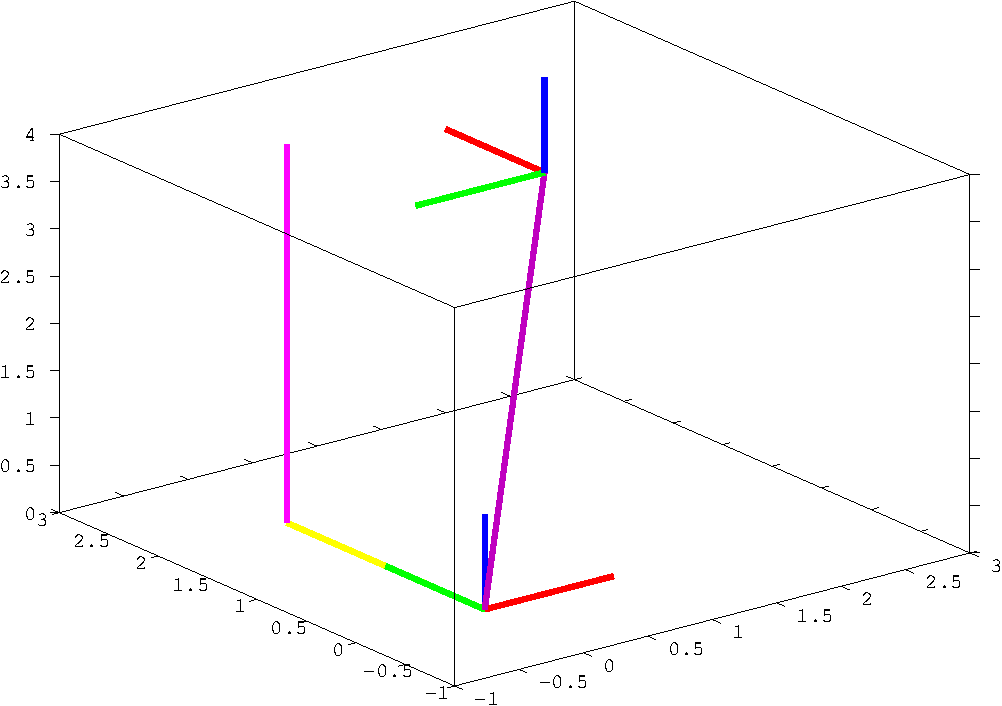
\includegraphics[width=0.95\textwidth]{part3/3d/FIG/3d/mozzi90.pdf}
\begin{picture}(0,0)(130,0)
\scriptsize{
\put(24,16){${\bm e}_2$}
\put(60,14){${\bm e}_1$}
\put(38,35){${\bm e}_3$}
\put(22,77){${{{\bm e}_2}_{R}}$}
\put(28,96){${{{\bm e}_1}_{R}}$}
\put(48,104){${{{\bm e}_3}_{R}}$}
\put(43,60){${\bm s}$}
\put(18,28){${\bm x}$}
\put(6,54){\rotatebox{90}{$\scriptscriptstyle{{\rm Mozzi}}$}}
\put(9,94){${\mu}$}
}
\end{picture}
\vskip .3cm
      \caption{\em
Asse del Mozzi con ${{\bm s}}=(2,2,4)^T$, $\theta=\psi=0$, $\phi=90^{\circ}$.
Posizione asse ${\bm x}=(0,2,0)^T$, angolo di rotazione elicoidale $\xi=90^{\circ}$.
}
 \label{fig:mozzi90}
\end{minipage}\hfill
\begin{minipage}[b]{0.45\textwidth}
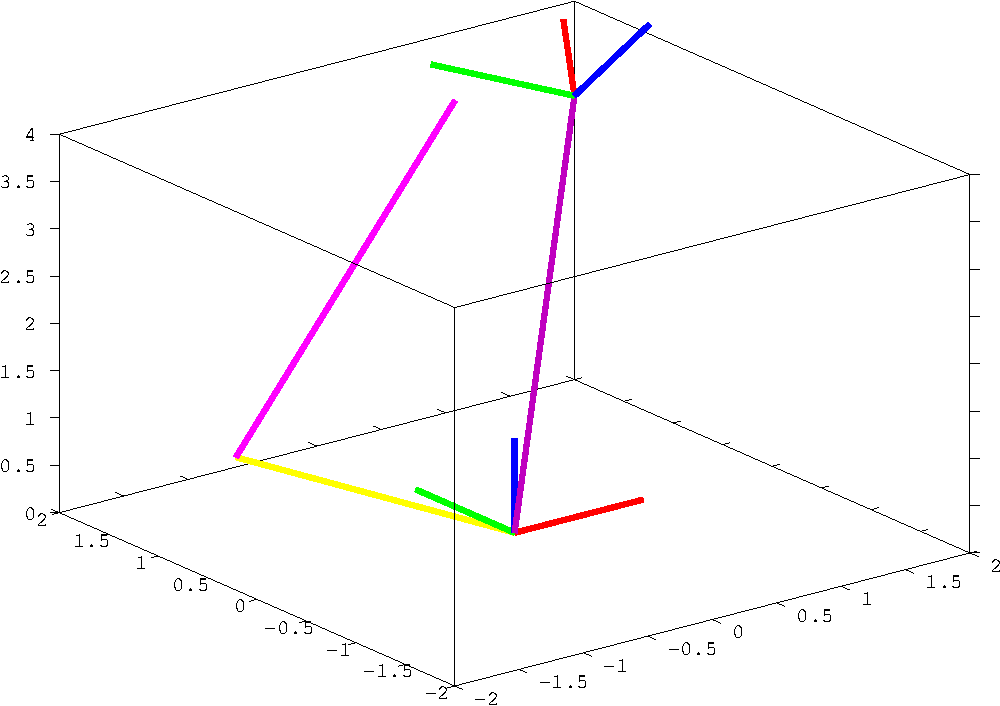
\includegraphics[width=0.95\textwidth]{part3/3d/FIG/3d/mozzi303030.pdf}
\begin{picture}(0,0)(130,0)
\scriptsize{
\put(32,36){${\bm e}_2$}
\put(69,27){${\bm e}_1$}
\put(45,43){${\bm e}_3$}
\put(29,102){${{{\bm e}_2}_{R}}$}
\put(52,110){${{{\bm e}_1}_{R}}$}
\put(72,106){${{{\bm e}_3}_{R}}$}
\put(52,75){${\bm s}$}
\put(12,30){${\bm x}$}
\put(13,53){\rotatebox{60}{$\scriptscriptstyle{{\rm Mozzi}}$}}
\put(35,92){${\mu}$}
}
\end{picture}
      \caption{\em
Asse del Mozzi con ${{\bm s}}=(2,2,4)^T$, $\theta=\psi=\phi=30^{\circ}$.
Posizione asse ${\bm x}=(-1.19, 1.26, 0.64)^T$, angolo di rotazione
elicoidale $\xi=66.45^{\circ}$.
      }
 \label{fig:mozzi303030}
\end{minipage}
\end{figure}

\noindent Le figure \ref{fig:mozzi90} e \ref{fig:mozzi303030} dovrebbero
dare un'idea dell'asse dello spostamento elicoidale $\mu$ per due casi di
spostamento rigido tridimensionale. Il primo caso, quello rappresentato
in figura \ref{fig:mozzi90}, riporta una traslazione della 
terna e una rotazione molto semplice, la quale avviene nel piano
$x-y$, attorno all'asse $z$, ed \`e pari a $90^{\circ}$ in senso
antiorario. In questo caso, la retta $\mu$ giace in una posizione 
ragionevolmente intuitiva, e questo ci serve da conforto dopo tutte
le avventure matematiche affrontate. La situazione rappresentata 
invece in figura \ref{fig:mozzi303030}, a fronte di una traslazione
 dalla terna di riferimento identica a quella del caso precedente,
prevede di applicare a tale terna le rotazioni, 
esprimibili in termini di angoli di Eulero, $\theta=\psi=\phi=30^{\circ}$.
In questo frangente, l'intuizione, almeno di chi scrive, si perde.
\`E vero che, in questa figura, l'asse del {\em Mozzi} somiglia a quello
dei ``mappamondi'' sferici, e il vettore ${\bm x}$ al supporto di tale asse,
ma siamo comunque obbligati ad accordare molta fiducia alla
formulazione matematica che abbiamo utilizzato per 
concedere, alla retta  $\mu$,
le caratteristiche di asse dello spostamento elicoidale.
\vskip .4cm
\footnotesize
\noindent I calcoli eseguiti per disegnare le figure \ref{fig:mozzi90} e
\ref{fig:mozzi303030} ci mettono a disposizione, in versione numerica,
gli oggetti che compaiono nelle relazioni matematiche test\'e esposte, e
ci sembrava un peccato non riportane alcuni, che potrebbero essere di aiuto
a qualche studente volenteroso di percorrere lo stesso cammino.
Proponiamo esclusivamente le quantit\`a legate alla figura
\ref{fig:mozzi303030}, che riteniamo maggiormente significative.
Per gli angoli di Eulero, precessione, nutazione e rotazione, come gi\`a
accennato, abbiamo $\theta =  \psi=\phi=0.52360$ rad. Quindi
\begin{equation}
{\bm R}=\left( \begin{array}{ccc}
0.53349 & -0.80801 &  \phantom{-}0.25000\\
0.80801 &  \phantom{-}0.39952 & -0.43301\\
0.25000 &  \phantom{-}0.43301 &  \phantom{-}0.86603\\
\end{array}
\right)
, 
{\bm H}=\left( \begin{array}{ccc}
\phantom{-}0.62325i & - 0.62325i &  0.47235\\
\phantom{-}0.70711  &   \phantom{-}0.70711  &  0\\
-0.3340i &   \phantom{-}0.33400i &  0.88141\\
\end{array}
\right).
\nonumber
\end{equation}
\noindent Gli autovalori sono  $\lambda_1=0.39952 + 0.91672i$, 
$\lambda_2=0.39952 - 0.91672i$ e $\lambda_3= 1$. Il vettore di traslazione,
che vale ${{\bm s}}=(2,2,4)^T$, nella base costituita dagli autovettori
di ${\bm R}$ vale ${{\bm s}'}=(1.4142 - 0.2445i, 1.4142 + 0.2445i, 3.5889)^T$.
\noindent Dopo le proiezioni su $\sigma$ abbiamo
\begin{equation}
\tilde{\bm s}'_{\sigma}= \left(\begin{array}{c}
1.4142 - 0.2445i\\
1.4142 + 0.2445i\\
\end{array}
\right),
\tilde{\bm R}'_{\sigma}=\left( \begin{array}{cc}
0.39952 + 0.91672i &  0\\
0 & 0.39952 - 0.91672i\\
\end{array}
\right).
\nonumber
\end{equation}
\noindent Infine abbiamo, per la posizione di $\mu$,
$\tilde{\bm x}'=(0.89374 + 0.95725i, 0.89374 - 0.95725i)^T$ e 
${\bm x}=( -1.19322, 1.26394, 0.63945)^T$.

\vskip .4cm

\normalsize
\noindent Le cose non vanno diversamente quando gli spostamenti sono
infinitesimali, e in tal caso l'asse del {\em Mozzi} si chiama anche
{\em asse d'istantanea  rotazione}\index{asse!di istantanea rotazione}.
Le superfici rigate disegnate dalla sequenza
degli assi d'istantanea rotazione, sia nel sistema fisso sia in quello
mobile, godono di interessanti propriet\`a, analoghe a quelle delle polari nel
moto piano, \cite{sesini1}, pag. 86.

\noindent Proponiamo un'ultima considerazione, di importanza marginale in questa gi\`a
troppo lunga digressione.
Anche nel caso del moto in tre dimensioni, come gi\`a visto per
il caso piano, le velocit\`a si possono esprimere surrogando
il prodotto 
${\bm \Omega}{\bm z}_{\scriptscriptstyle{P(\Gamma)}}$ con un prodotto
vettoriale e si pu\`o riscrivere la \ref{e115_app11} come segue
\begin{equation}
{\bm v}_{\scriptscriptstyle{P}}=
{\bm v}_{\scriptscriptstyle\Gamma}+
{\bm \omega}\times {\bm z}_{\scriptscriptstyle{P}}\,,
\label{e120_app11}
\end{equation}
\noindent dove il vettore $\bm \omega$ ha le seguenti componenti
\begin{equation}
{\bm\omega}=\left( \begin{array}{c}
\omega{{\scriptscriptstyle{2,3}}}\\
\omega{{\scriptscriptstyle{3,1}}}\\
\omega{{\scriptscriptstyle{1,2}}}
\end{array}
\right)\,.
\label{e119_app11}
\end{equation}
\noindent L'equivalenza del prodotto matriciale della \ref{e115_app11} col prodotto
vettoriale della \ref{e120_app11} dipende strettamente dalla forma particolare
di $\bm \Omega$, e la verifica di questa affermazione \`e lasciata al paziente lettore.
Rimarchiamo semplicemente che la comodit\`a insita nell'introduzione del vettore
velocit\`a angolare $\bm \omega$ rende il suo uso frequentissimo. 
La possibilit\`a di rappresentare le rotazioni infinitesime, quindi 
le velocit\`a angolari, mediante un vettore \`e ristretta per\`o allo spazio tridimensionale.
Infatti con solo due dimensioni, l'angolo di rotazione \`e unico e occuperebbe
le caselle libere della matrice antisimmetrica $2\times2$
di rotazione.
Ci sarebbe perci\`o troppo spazio in un vettore a due dimensioni. \`E vero che 
abbiamo utilizzato la rappresentazione vettoriale della velocit\`a angolare
anche nel caso di moto piano, ma il vettore $\bm \omega$ risulta non appartenere al piano stesso.
Del resto
risulta cos\`i difficile concepire uno spazio che non sia quello tridimensionale!
Viene sempre la tentazione di trattare gli spazi con numero di dimensioni inferiore
a tre come se fossero immersi nel tridimensionale stesso.
Qualora poi il numero delle dimensioni $n$ dello spazio fosse maggiore
di tre,
si otterrebbe, per la matrice di 
rotazione, un numero di componenti ``libere'' pari a $(n^2 - n)/2$.
Quindi, per uno spazio quadridimensionale si dovrebbero considerare sei componenti di rotazione,
numero decisamente eccessivo per potere
entrare in un vettore quadridimensionale.
\endinput
